\documentclass[]{article}
\usepackage{graphicx}
\usepackage[space]{grffile}
\usepackage{subfig}
\graphicspath{ {./roc_curves/} }

%opening
\title{Transfer Learning Using Convolutional Neural Networks to Detect Spoofs in Fingerprints}
\author{Chris Denniston}

\begin{document}

\maketitle

\begin{abstract}

\end{abstract}
\section{Introduction}

\section{Formulation of Problem}
%1. Define the problem to be considered in detail. Typically this section might begin with something like: LConsider a packetradio system consisting of a single central repeater surrounded by user terminals. Each user transmits packets to the central repeater using a slotted ALOHA protocol[1]. The transmissions from all users are assumed to be on the same frequency...N The discussion should proceed in this way until the problem is completely defined.
%2. Define all terminology and notation used. Usually the terminology and notation are defined along with the problem itself.
%3. Develop the equations on which your results will be based and/or describe any experimental systems.
Detection of impostor fingerprints are an important part of a fingerprint based biometric system. These impostor and fake fingerprints are commonly called "spoofs" It is not enough that the system can tell apart one person from another, but also must be able to tell apart fake fingerprints from real fingerprints to inspire real confidence in it's users. Spoof fingerprints can be made from common household materials and more and more material's are appearing which can be used to make these spoofs. Because of this it is also important that a spoof detection system also can detect spoofs when novel types of materials are used on it. 

A neural network may be used to solve this complex classification problem as it has the ability to learn from a large variety of samples and draw complex decision boundaries. \cite{book} (Citation?) Neural networks are expensive to train for complex problems involving large dimensional data, such as images. It is possible to take a pre-trained general image classification neural network and reapply it to this classification task. This enables a much quicker training time and more accurate results than could be achieved by a small team. 

Convolutional Neural Networks provide a framework 
\section{Results}
%This section presents the detailed results you have obtained. If the paper is theoretical, you will probably show curves obtained from your equations. If the paper is experimental, you will be presenting curves showing the measurement results. In order to choose the proper curves to present, you must first be clear what point you are trying to convey to the reader. The curves can then be chosen to illustrate this point. Whether your paper is theoretical or experimental, you must provide a careful interpretation of what your results mean and why they behave as they do.
\section{Conclusion}
%Section IV: Conclusion This section should summarize what has been accomplished in the paper. Many readers will read only the Introduction and Conclusion of your paper. The Conclusion should be written so they can be understood by someone who has not read the main work of the paper.
\section{Reference}
\section{Appendix}
\begin{figure}[!ht]
     \subfloat[Testing\label{subfig-1:dummy}]{%
       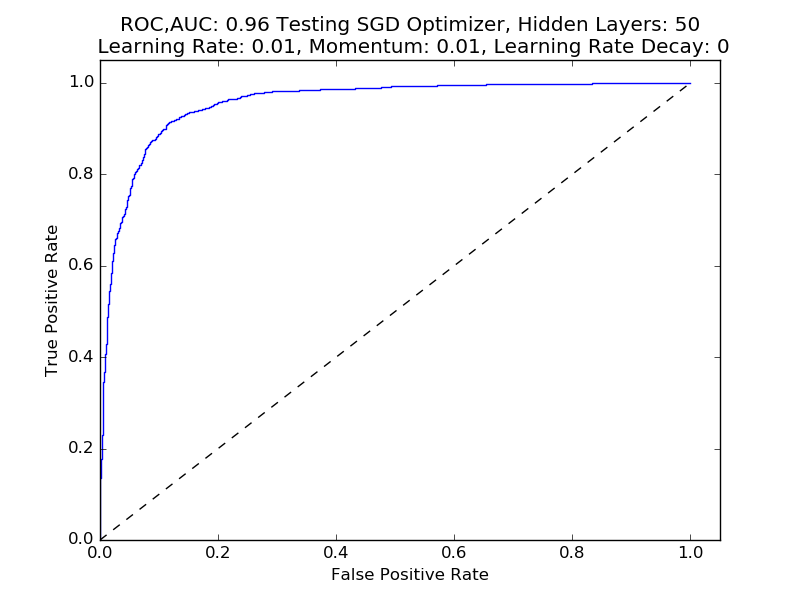
\includegraphics[width=0.5\textwidth]{/home/octopuscabbage/code/NeuralAndAdaptiveSystemsFinal/roc_curves/SGD Optimizer, Hidden Layers: 50 Learning Rate: 0.01, Momentum: 0.01, Learning Rate Decay: 0/ROC,AUC: 0.96 Testing SGD Optimizer, Hidden Layers: 50 Learning Rate: 0.01, Momentum: 0.01, Learning Rate Decay: 0}
     }
     \hfill
     \subfloat[Validation\label{subfig-2:dummy}]{%
       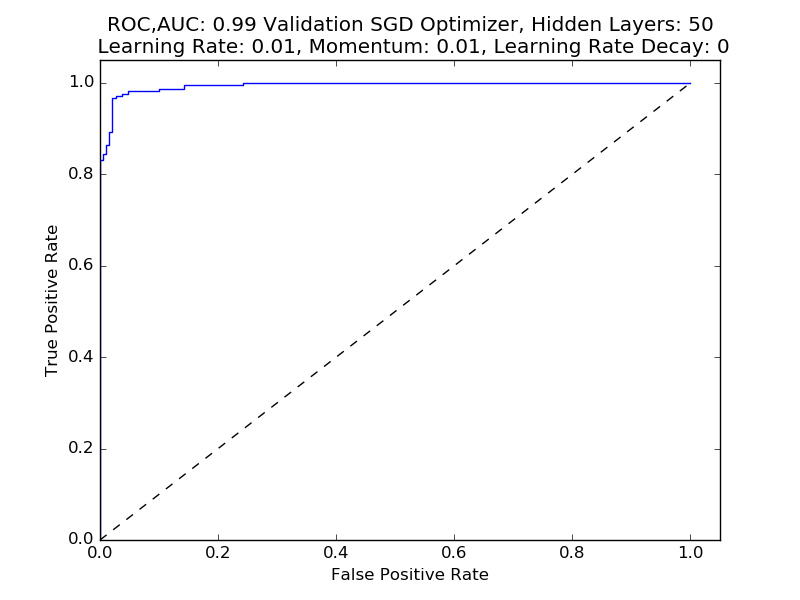
\includegraphics[width=0.5\textwidth]{/home/octopuscabbage/code/NeuralAndAdaptiveSystemsFinal/roc_curves/SGD Optimizer, Hidden Layers: 50 Learning Rate: 0.01, Momentum: 0.01, Learning Rate Decay: 0/ROC,AUC: 0.99 Validation SGD Optimizer, Hidden Layers: 50 Learning Rate: 0.01, Momentum: 0.01, Learning Rate Decay: 0}
     }
     \caption{ROC Curves For Training On All Samples}
     \label{fig:dummy}
   \end{figure}

\begin{figure}[!ht]
     \subfloat[Gelatine\label{subfig-3:dummy}]{%
       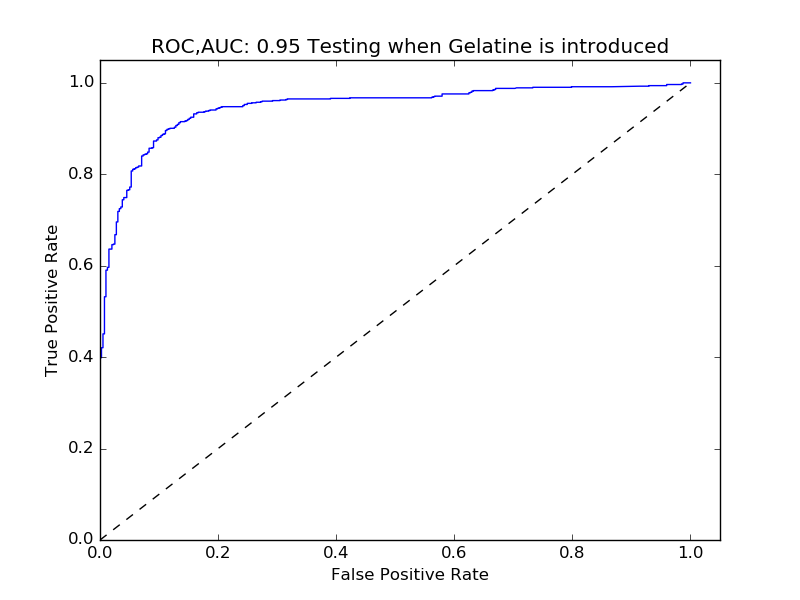
\includegraphics[width=0.5\textwidth]{/home/octopuscabbage/code/NeuralAndAdaptiveSystemsFinal/roc_curves/Gelatine/ROC,AUC: 0.95 Testing when Gelatine is introduced}
     }
     \hfill
     \subfloat[Latex\label{subfig-4:dummy}]{%
       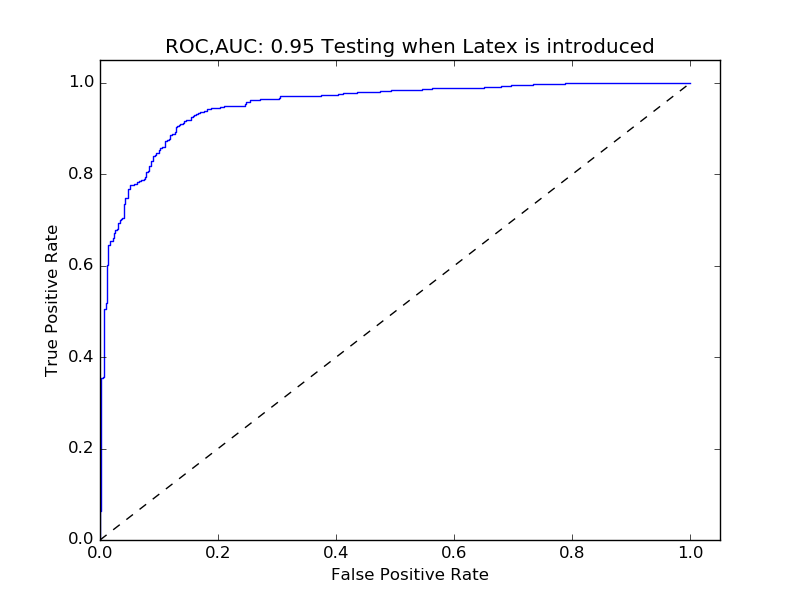
\includegraphics[width=0.5\textwidth]{/home/octopuscabbage/code/NeuralAndAdaptiveSystemsFinal/roc_curves/Latex/ROC,AUC: 0.95 Testing when Latex is introduced}
     }
     \hfill
     \subfloat[Playdoh\label{subfig-5:dummy}]{%
            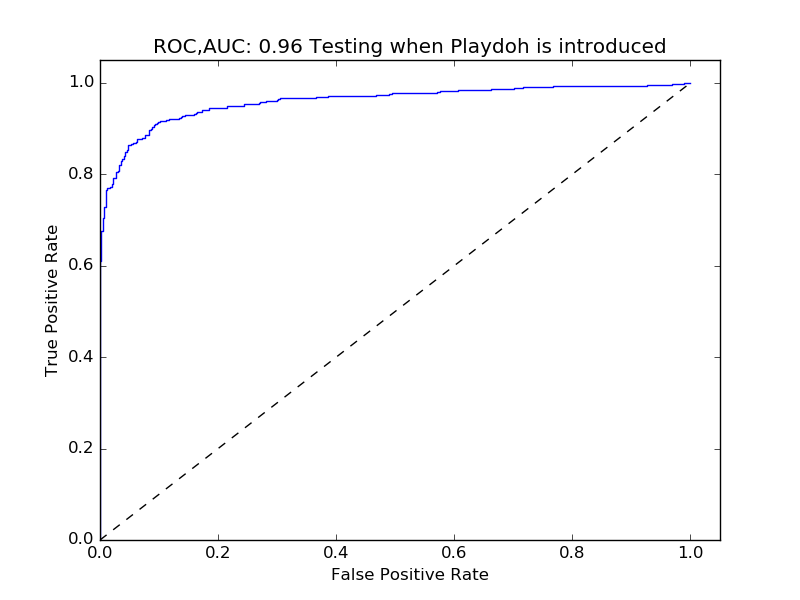
\includegraphics[width=0.5\textwidth]{/home/octopuscabbage/code/NeuralAndAdaptiveSystemsFinal/roc_curves/Playdoh/ROC,AUC: 0.96 Testing when Playdoh is introduced}
    }
    \hfill
    \subfloat[Silicone\label{subfig-6:dummy}]{%
    	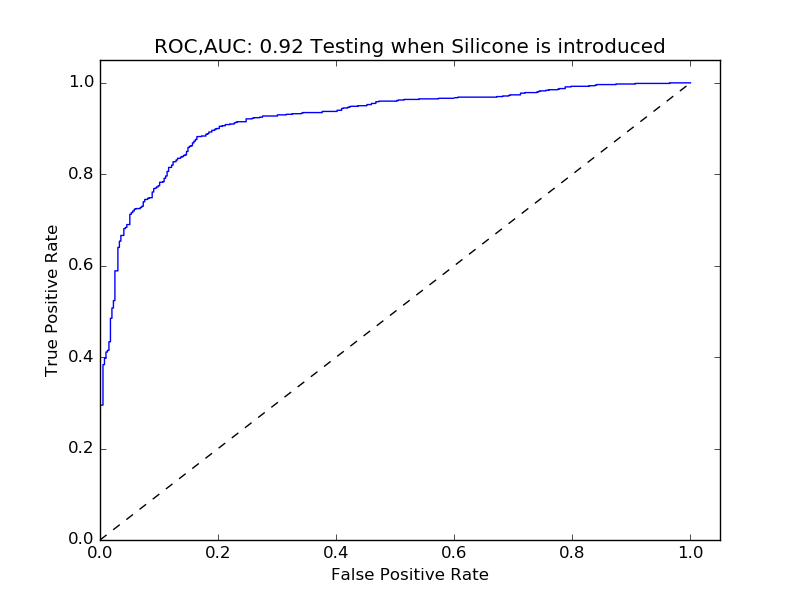
\includegraphics[width=0.5\textwidth]{/home/octopuscabbage/code/NeuralAndAdaptiveSystemsFinal/roc_curves/Silicone/ROC,AUC: 0.92 Testing when Silicone is introduced}
    }
    \subfloat[Wood Glue\label{subfig-7:dummy}]{%
         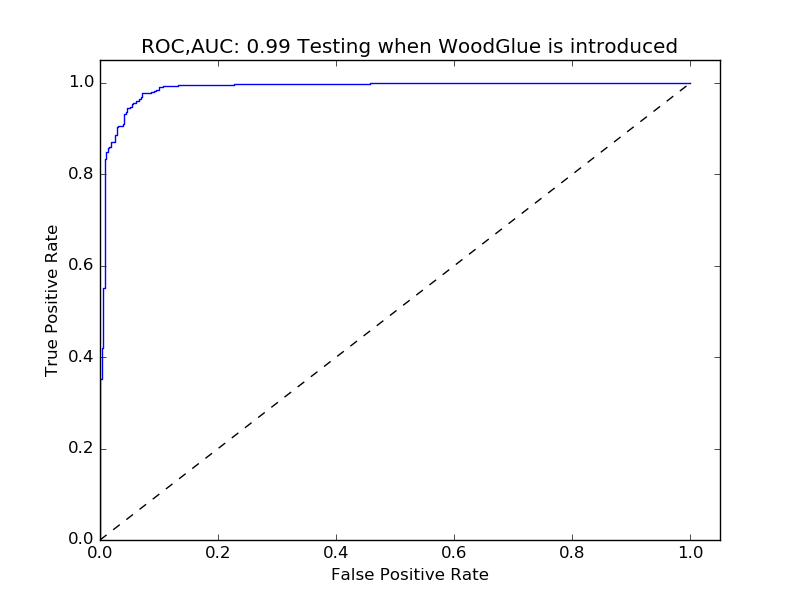
\includegraphics[width=0.5\textwidth]{/home/octopuscabbage/code/NeuralAndAdaptiveSystemsFinal/roc_curves/WoodGlue/ROC,AUC: 0.99 Testing when WoodGlue is introduced}
     }
     \caption{ROC Curves When Novel Spoofs Are Introduced}
     \label{fig-2:dummy}
   \end{figure}
   \nocite{*}
\bibliographystyle{ieeetr}
\bibliography{/home/octopuscabbage/code/NeuralAndAdaptiveSystemsFinal/report/bib.bib}
\end{document}

